\documentclass{article}
\usepackage[utf8]{inputenc}
\usepackage{graphicx}
\usepackage{titlepic}
\usepackage{caption}
\usepackage{subcaption}
% \documentclass{beamer}

\newcommand{\namesigdate}[2][5cm]{%
  \begin{tabular}{@{}p{#1}@{}}
    #2 \\[0.4\normalbaselineskip] \hrule \\[0pt]
    {\small } \\[2\normalbaselineskip] 
  \end{tabular} 
}

\title{\textbf{Hybrid Logical Clocks}}
\author{Vaibhav Bhagee (2014CS50297)}
\date{}

\begin{document}
\maketitle

\begin{center}
\noindent\rule{3.2cm}{0.4pt} 
\end{center}

    \section{Introduction}

    Ordering of events in a distributed system is of utmost importance when arguing about causality and correctness, with clocks lying at the very heart of that. Most of the work done in distributed computing completely disregards the physical notion of time and is based on its logical notion. While that helps us track causality of events in a system, most physical implementations can't entirely do away with the physical notion of time in order to support real time operations and queries. \\

    Physical clocks are also known to have issues, related to non monotonosity and drift, which makes them infeasible for causality tracking. In this report, we look at Hybrid Logical Clocks\cite{hlc}, which help us get the best out of both worlds. HLC timestamps enable tracking causality of events in a distributed system, while being a bounded approximation to the system time. Further properties of HLCs along with their applications, have been discussed is greater detail in the subsequent sections.

    \section{Motivation}

    There have been various attempts made towards formulation of algorithms, used to timestamp events in a distributed system. A key requirement from such an algorithm is that the timestamps should be such that they should at least enable tracking causal dependencies among the events of the system. \\

    Let us denote the timestamp of an event $e$ as $t.e$. Then, in particular, for two events $e$ and $f$, $$e \prec f \rightarrow t.e < t.f$$ where $\prec$ is the $happens\ before$ relation.

    \subsection{Logical and Vector Clocks}

    Logical clocks\cite{lc} proposed by Lamport and Vector clocks\cite{vc} proposed by Mattern, timestamp the events based on the logical notion of time. They do away with system clocks and the physical notions of time. Both the algorithms enable tracking of causal dependencies as described above. Vector clocks further ensure that for two events $e$ and $f$, $$e \prec f \iff t.e < t.f$$ where $\prec$ is the $happens\ before$ relation. \\

    However, real time deployments of distributed systems cannot rely solely on logical and vector clocks. Many systems like distributed databases require answering of queries which rely on physical time. An example of such a query in a system which tracks jobs running on a group of virtual machines could involve returning the IDs of the events which failed in the part hour. In such a scenario, logical clocks become incapable of answering such queries. \\

    Also, vector clocks have an associated space overhead, where the storage is proportional to the number of processes in the system. Many algorithms have since been proposed which try to bound the storage of the vector clock timestamps. While those algorithms successfully bound the storage costs, the trade of has to be made with an increased computation cost, while tracking the causal dependencies.

    \subsection{Physical Clocks}

    Physical clocks, unlike logical clocks, take into account the system time at the nodes. The vanilla physical clocks suffer from issues of $drift$ and $non\ monotonosity$. Due to the different rates at which the clocks at different nodes of the system might tick, the latter may eventually drift apart. This leads to a periodic requirement for $clock\ synchronisation$. \\

    While synchronisation resolves the problem of drift, it leads to a new problem of non monotonosity. Due to the periodic synchronisation, it may so happen that the timestamp at a later stage of the protocol, might turn out to be lesser that the timestamp at an earlier stage. Thus, it can happen that for two events $e$ and $f$, the event $e\ \prec\ f$ but $l.e\ >\ l.f$. This leads to periods of uncertainty and subsequently leading to inability to order events.

    \subsection{True Time}

    True time is proposed by Google, as a part of their strongly consistent distributed database called Spanner\cite{spanner}. Spanner utilises GPS and atomic clocks for tight clock synchronisation. This leads to a very low clock drift. However, this can still have small periods of uncertainty. True time, exposes this uncertainty as an abstraction. \\

    The timestamp allotted by True time is a tuple $(earliest,\ latest)$, which specifies the bounds in which the exact timestamp could lie. If the intervals for two events overlap, it leads to uncertainty. To overcome this limitation, Spanner uses the idea of inducing delays. This means that if an event $e\ \prec\ f$ and the timestamps of $e$ and $f$ are not disjoint, then we delay $f$ to a point where $f.earliest\ >\ e.greatest$. \\

    To overcome the limitations of the algorithms, as pointed out earlier, the authors propose Hybrid Logical Clocks.

    \section{Hybrid Logical Clocks}

    For every event $e$, the HLC associates a timestamp value $t$ such that $t\ =\ (l,c)$. Here $l$ is the physical component of the timestamp and $c$ is the logical component. While preserving the causal ordering property of logical clocks, the HLC timestamps are withing an $\epsilon$ bound of the physical clock timestamps. The updates to the HLC timestamps are monotonic and the space requirement for the HLC timestamp is bounded.

    \subsection{Algorithm}

    At an abstract level, for an event $f$, the HLC timestamp at $f$ depends on the HLC timestamp at the predecessor(s) of $f$. If the physical clock timestamp at the event $f$ has not caught up with the value of the physical component of the HLC timestamp at the predecessor, then the causal component of the HLC timestamp at $f$ is incremented by 1, to capture the causality while the physical component of the latter is kept equal to the corresponding component of the predecessor. However, if the physical timestamp at $f$ manages to catch up, as discussed before, then the causal component gets reset to 0. A formal algorithm is given in figure 1. 

    \begin{figure}[h!]
        \begin{center}
        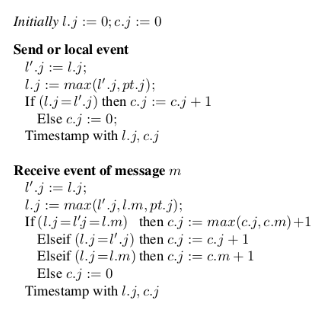
\includegraphics[resolution=125]{algorithm.png}
        \end{center}
        \caption{HLC Algorithm}
    \end{figure}

    \subsection{Properties}

    After having looked at the HLC algorithm, we will now look at the properties satisfied by the HLC timestamps. We will discuss about the reasoning in brief. The interested readers can take a look at the technical paper, for the detailed arguments. \\

    \noindent \textbf{Theorem 1:} For any two events $e$ and $f$, $$e \prec f \rightarrow (l.e,c.e) < (l.f,c.f)$$ \\

    This can be formally proved, directly from the algorithm. Intuitively, if $e\ \prec\ f$, then due to the use of the $max$ function, we can show that $l.e\ \leq\ l.f$. Now, if $l.e\ <\ l.f$ then the consequent becomes true. Otherwise if $l.e\ =\ l.f$ then, by the algorithm, $c.f\ =\ c.e\ +\ 1$. \\

    \noindent \textbf{Theorem 2:} For any event $f$, $l.f\ \geq\ pt.f$ \\

    This is also a direct consequence of the algorithm. \\

    \noindent \textbf{Theorem 3:} $l.f$ denotes the maximum clock value that $f$ is aware of. Thus, $$l.f > pt.f \rightarrow (\exists g: g \prec f \land pt.g = l.f)$$ \\

    This can be proved using induction. For the induction step, we consider the cases when $f$ is a send event or a receive event. In the former case, let $e$ be the event just preceding the send. Thus, for $e$ we have $$l.e > pt.e \rightarrow (\exists g: g \prec e \land pt.g = l.e)$$ Now, if $l.f\ >\ pt.f$, then, according to the algorithm, we have $l.e\ =\ l.f\ =\ pt.g$. The proof for the latter case is similar to the proof of the former. \\

    \noindent \textbf{Theorem 4:} For any event $f$, $|l.f\ -\ pt.f|\ <\ \epsilon$ \\

    We use the clock synchronisation constraints for the physical clocks, which ensure that there cannot exist events $g$ and $f$ such that $g\ \prec\ f$ and $pt.g\ >\ pt.f\ +\ \epsilon$. Also, using the previous theorem we have $$l.f > pt.f \rightarrow (\exists g: g \prec f \land pt.g = l.f)$$ But, $pt.g\ \leq\ pt.f\ +\ \epsilon$. Thus, $l.f\ \leq\ pt.f\ +\ \epsilon$. \\

    \noindent \textbf{Theorem 5:} For any event $f$, $c.f\ =\ k\ \land\ k\ >\ 0\ \rightarrow$ $\exists$ a chain of $k$ events which causally precede the event $f$ in the system, having the same value of the physical component of the HLC. \\

    This property is similar to the property of Lamport clock timestamps. This can be proved using induction, as the authors have suggested in the paper. Intuitively, we can again split the proof into cases when $f$ is a send or a receive event and both the cases are proven similarly. For the send case, let $e$ be the event which causally precedes $f$. Then, if $l.e\ =\ l.f$, we have $c.f\ =\ c.e\ +\ 1$ and $e$ satisfies the induction hypothesis. As mentioned, the proof of the case when $f$ is a receive event, is similar. \\

    \noindent \textbf{Theorem 6:} For any event $f$, $c.f\ \leq\ N*(\epsilon\ +\ 1)$ \\

    This proof can be done using the clock synchronisation constraints again. Using the constraints, we can conclude that for all events $e$ having $l.e\ =\ l.f$, the event would have happened at a physical time lying in $[l.f,\ l.f+\epsilon]$. Also, at any node, the number of events which can happen in this time interval is at most $\epsilon\ +\ 1$. This is due to the constraint that the physical clock gets incremented by at least $1$ between two subsequent events on the same node. Hence, for $N$ processes, the bound becomes $N*(\epsilon+1)$. \\

    % \section{Applications of HLCs}

    

    % \section{Extensions and research directions}    

\bibliographystyle{acm}
\bibliography{references}

\end{document}